\documentclass[12pt,oneside,reqno]{article}
\usepackage{polski}
\usepackage[T1]{fontenc}%polskie znaki
\usepackage[utf8]{inputenc}%polskie znaki
\usepackage[left=3cm,right=3cm,top=3cm,bottom=3cm]{geometry}
% \usepackage{scrextend}
\usepackage{graphicx}
\usepackage{hyperref}
\usepackage{enumitem}
\usepackage{caption}
\usepackage{amsmath}
\usepackage{amsfonts}
\usepackage{float}
\usepackage{dirtytalk}
\usepackage{listings}
\usepackage{color}
\usepackage{tabularx}
\usepackage{indentfirst}

\newcommand{\tabitem}{~~\llap{\textbullet}~~}
\renewcommand*{\thesection}{\arabic{section}}
\newenvironment{code}{\captionsetup{type=listing}}{}
\makeatletter
\newcommand{\linia}{\rule{\linewidth}{0.4mm}}

\definecolor{mygreen}{rgb}{0,0.6,0}
\definecolor{mygray}{rgb}{0.5,0.5,0.5}
\definecolor{mymauve}{rgb}{0.58,0,0.82}

\lstset{ 
  backgroundcolor=\color{white},   % choose the background color; you must add \usepackage{color} or \usepackage{xcolor}; should come as last argument
  basicstyle=\footnotesize,        % the size of the fonts that are used for the code
  breakatwhitespace=false,         % sets if automatic breaks should only happen at whitespace
  breaklines=true,                 % sets automatic line breaking
  captionpos=b,                    % sets the caption-position to bottom
  commentstyle=\color{mygreen},    % comment style
  deletekeywords={...},            % if you want to delete keywords from the given language
  escapeinside={\%*}{*)},          % if you want to add LaTeX within your code
  extendedchars=true,              % lets you use non-ASCII characters; for 8-bits encodings only, does not work with UTF-8
  firstnumber=1,                % start line enumeration with line 1000
  frame=single,	                   % adds a frame around the code
  keepspaces=true,                 % keeps spaces in text, useful for keeping indentation of code (possibly needs columns=flexible)
  keywordstyle=\color{blue},       % keyword style
  language=[x86masm]Assembler,                 % the language of the code
  morekeywords={*,...},            % if you want to add more keywords to the set
  numbers=left,                    % where to put the line-numbers; possible values are (none, left, right)
  numbersep=5pt,                   % how far the line-numbers are from the code
  numberstyle=\tiny\color{mygray}, % the style that is used for the line-numbers
  rulecolor=\color{black},         % if not set, the frame-color may be changed on line-breaks within not-black text (e.g. comments (green here))
  showspaces=false,                % show spaces everywhere adding particular underscores; it overrides 'showstringspaces'
  showstringspaces=false,          % underline spaces within strings only
  showtabs=false,                  % show tabs within strings adding particular underscores
  stepnumber=1,                    % the step between two line-numbers. If it's 1, each line will be numbered
  stringstyle=\color{mymauve},     % string literal style
  tabsize=2,	                   % sets default tabsize to 2 spaces
  title=\lstname                   % show the filename of files included with \lstinputlisting; also try caption instead of title
}

\renewcommand{\maketitle}{\begin{titlepage}
    \begin{figure}[H]
    \centering
    
\includegraphics[width=50px]{images/pwrlogo.jpg}
    \label{fig:logo}
    \end{figure}
    \begin{center}   
        Wydział Elektroniki
    \end{center}
    \vspace{1cm}
    \begin{center}
        \Large \textsc{Organizacja i Architektura Komputerów}
    \end{center}
    \vspace{1cm}
    \noindent\linia
    \begin{center}
      \Huge \textsc{\@title}
         \end{center}
     \linia
    \vspace{2cm}
    \begin{flushright}
    \small Autorzy:\\
    \normalsize \textbf{\@author}
        \vspace{1cm}
        \vspace{3cm}
        {\small Prowadzący projekt:}\\
        \textbf{Dr inż. Piotr Patronik}
    \end{flushright}
    \begin{center}
    Wrocław \@date
    \end{center}
  \end{titlepage}
}
\makeatother
\author{Maja Bojarska \\
        Paweł Sajewicz \\}
\title{Implementacja fizyczna układów cyfrowych}
\begin{document}
\maketitle
\clearpage
\tableofcontents
\clearpage

\setlength{\parskip}{0.5em}

\section{Wstęp}
\subsection{Cele projektu}
Cel ogólny: Synteza logiczna i fizyczna sumatora prefiksowego z wykorzystaniem narzędzi Yosys/Qflow.

Cele szczegółowe:
\begin{itemize}
    \item Analiza literatury w zakresie narzędzia Yosys/Qflow.
    \item Wybór architektury 6-bitowego sumatora prefiksowego i jej zapis w strukturalnym języku Verilog.
    \item Implementacja testu wyczerpującego.
    \item Synteza logiczna układu z wykorzystaniem Yosys.
    \item Synteza fizyczna układu z wykorzystaniem Qflow.
\end{itemize}

\subsection{Użyte technologie}
\begin{itemize}
    \item Ubuntu 20.04 \cite{ubuntu} - system operacyjny GNU/Linux.
    \item Verilog 2005 \cite{ieee-verilog} - język opisu sprzętu.
    \item Icarus Verilog 10.3 \cite{iverilog} - symulator języka Verilog.
    \item Pytest \cite{pytest} - framework do tworzenia testów.
    \item Yosys 0.9 \cite{yosys} - narzędzie do syntezy Verilog.
    \item Qflow 1.3 \cite{qflow} - narzędzie do syntezy układów cyfrowych.
\end{itemize}

\clearpage
\section{Podstawy}
\subsection{Sumatory prefiksowe}
W celu skonstruowania sumatora prefiksowego najpierw musimy poznać zależności wytwarzania przez nie sum oraz propagacji i generacji przeniesień. Prezentują je wzory \cite{szybkie-sumatory-2009}: 

$s_i=h_i\oplus c_i=h_i\oplus (G_{i-1:0}+P_{i-1:0}c_0)$,

$c_i=G_{i-1:0}+P_{i-1:0}c_0$,

$h_i=x_i\oplus y_i$,

\noindent gdzie $s_i$ to bit sumy na i-tej pozycji, $c_i$ - przeniesienia, $h_i$ - pół sumy, $G_{i-1:0}$ - generacji przeniesienia, $P_{i-1:0}$ - propagacji przeniesienia, $x_i$ - pierwszego składnika dodawania, $y_i$ drugiego składnika, a $c_0$ to przeniesienie z poprzedniej pozycji.

Węzeł sieci GP realizuje funkcję
\begin{equation}
(G_{HL}, P_{HL})=(G_H, P_H)\bullet(G_L, P_L)=(G_H+P_HG_L, _HP_L).
\label{formula:prefix-node}
\end{equation}

Zasada konstrukcji struktury GP:

\quad integracja funkcji $G_H$ i $P_H$ oraz $G_L$ i $P_L$ obejmujących sąsiadujące bloki H i L:
\begin{itemize}
    \item bloki H i L powinny być styczne,
    \item bloki H i L nie mogą być rozdzielone,
    \item bloki H i L mogą mieć część wspólną – funkcje $G_{HL}$ i $P_{HL}$ są nadmiarowe,
    \item regularne struktury dla $n=2^k$ wejść (pozycji),
    \item w innych przypadkach przyjąć $k=int(1+log_2n)$ i usunąć zbędne gałęzie (sieć integrującą $2^{k-1}$ pozycji połączyć siecią integrującą pozostałe wejścia).
\end{itemize}

\setlength{\parskip}{0em}
Przekształcenie prefiksowe Ladnera-Fischera (Sklansky’ego) \cite{szybkie-sumatory-2006}:\\

$P_{i:i}=x_i\oplus y_i , G_{i:i}=x_iy_i (i=0,1,\dots,n-1)\hfill G_{0:0}$\\

Poziom 1 $(i=0,1,\dots,2^{- 1}n-1)\hfill G_{1:0}$

$(G_{2i+1:2i},P_{2i+1:2i})=(G_{2i+1:2i+1}+P_{2i+1:2i+1}G_{2i:2i}, P_{2i+1:2i+1}P_{2i:2i})$\\

Poziom 2 $(i=0,1,\dots,2^{- 2}n-1; s=2,3)\hfill G_{3:0}, G_{2:0}$

$(G_{4i+s:4i},P_{4i+s:4i})=(G_{4i+s:4i+2}+P_{4i+s:4i+2}G_{4i+1:4i},P_{4i+s:4i+2}P_{4i+1:4i})$\\

Poziom 3 $(i=0,1,\dots,2^{- 3}n-1; s=4,5,6,7)\hfill G_{7:0} ,\dots,G_{4:0}$

$(G_{8i+s,8i},P_{8i+s,8i})=(G_{8i+s,8i+4}+P_{8i+s,8i+4}G_{8i+3,8i}, P_{8i+s,8i+4}P_{8i+3,8i})$\\

Poziom 4 $(i=0,1,\dots,2^{- 4}n-1; s=8,9,\dots,15)\hfill G_{15:0} ,\dots,G_{8:0}$

$(G_{16i+s,16i},P_{16i+s,16i})=(G_{16i+s,16i+8}+P_{16i+s,16i+8}G_{16i+7,16i},P_{16i+s,16i+8}P_{16i+7,16i})$

\dots

\setlength{\parskip}{0.5em}

\subsection{Yosys}
Yosys \cite{yosys} to oprogramowanie do syntezy Verilog HDL, które obsługuje ogromną większość możliwych do syntezy funkcji Verilog. Synteza HDL służy do tłumaczenia kodu języka opisu sprzętu Verilog HDL na układy cyfrowe. Yosys został zbudowany jako rozszerzalna platforma, dzięki czemu można go łatwo używać jako podstawy dla niestandardowych przepływów syntezy oraz jako środowisko do wdrażania i badań nad nowymi algorytmami syntezy. Yosys posiada szerokie wsparcie dla Verilog HDL i jest w stanie syntezować złożone projekty Verilog. \cite{yosys-manual}

Synteza jest automatyczną konwersją reprezentacji wysokiego poziomu obwodu na funkcjonalnie równoważną reprezentację niskiego poziomu obwodu. Rysunek \ref{fig:abstract} przedstawia różne poziomy abstrakcji i ich związek z różnymi rodzajami syntezy. Jak widzimy oprogramowanie Yosys odpowiada za syntezę behawioralną, RTL i logiczną.
\begin{figure}[H]
\centering
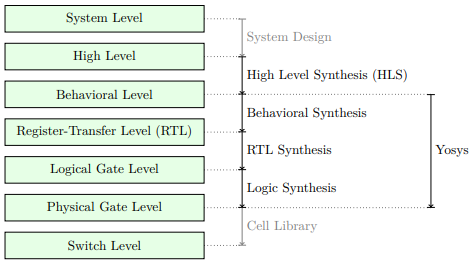
\includegraphics[width=350px]{images/abstract.jpg}
\caption{Różne poziomy abstrakcji i syntezy. \cite{yosys-manual}}\label{fig:abstract}
\end{figure}

\subsection{Qflow}
Qflow to kompletny łańcuch narzędzi do syntezy układów cyfrowych, czyli zestaw narzędzi i metod używanych do przekształcenia projektu układu napisanego w wysoko poziomowym języku behawioralnym, takim jak verilog lub VHDL, w układ fizyczny. Taki obwód może być kodem konfiguracji dla układu FPGA, takiego jak układ Xilinx lub Altera, który stałby się częścią ukształtowanego układu scalonego. \cite{qflow}

Qflow korzysta z szeregu narzędzi, każde jest odpowiedzialne za inną funkcję:
\begin{itemize}
    \item Yosys - parsowanie, synteza, optymalizacja i weryfikacja Verilog.
    \item Graywolf - rozmieszczenie komórek i pinów.
    \item Grouter - szczegółowy routing.
    \item Magic - przeglądanie, ekstrakcja, sprawdzanie DRC, generowanie GDS.
    \item Netgen - LVS (Layout vs. Schematic), weryfikuje czy otrzymany układ scalony odpowiada oryginalnemu schematowi obwodu w projekcie.
\end{itemize}
Proces syntezy obrazuje rysunek \ref{fig:synthesis}.
\begin{figure}[H]
\centering
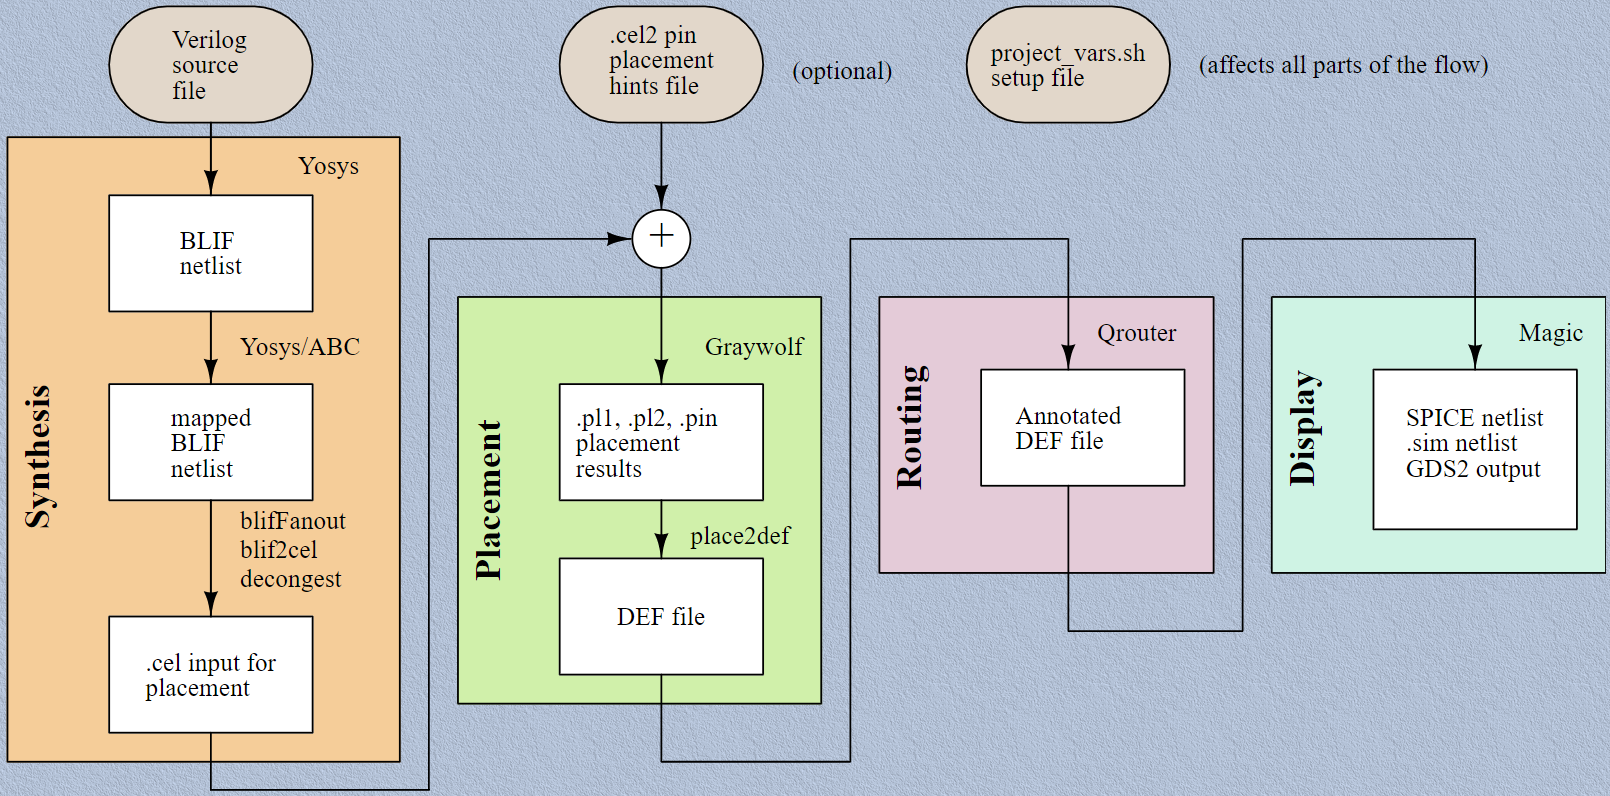
\includegraphics[width=\linewidth]{images/qflowsyn.jpg}
\caption{Proces syntezy z użyciem Qflow. \cite{opencircuitdesign-qflow}}\label{fig:synthesis}
\end{figure}

\clearpage
\section{Rozwiązanie}

\subsection{Architektura układu}

Przed rozpoczęciem opisu układu językiem Verilog, każdy z modułów został zaprojektowany w postaci układu, składającego się z bramek logicznych i/lub lub modułów. 

\subsubsection{Blok PG} 
\label{section:pg-block}

Blok PG realizuje funkcje logiczne generacji oraz propagacji, opisane funkcjami ze wzoru nr \ref{formula:pg}.

\begin{equation}
    \begin{cases}
      g = x*y\\
      p = x+y\\
      h = x\oplus y
    \end{cases}
    \label{formula:pg}
\end{equation}

\begin{figure}[H]
\centering
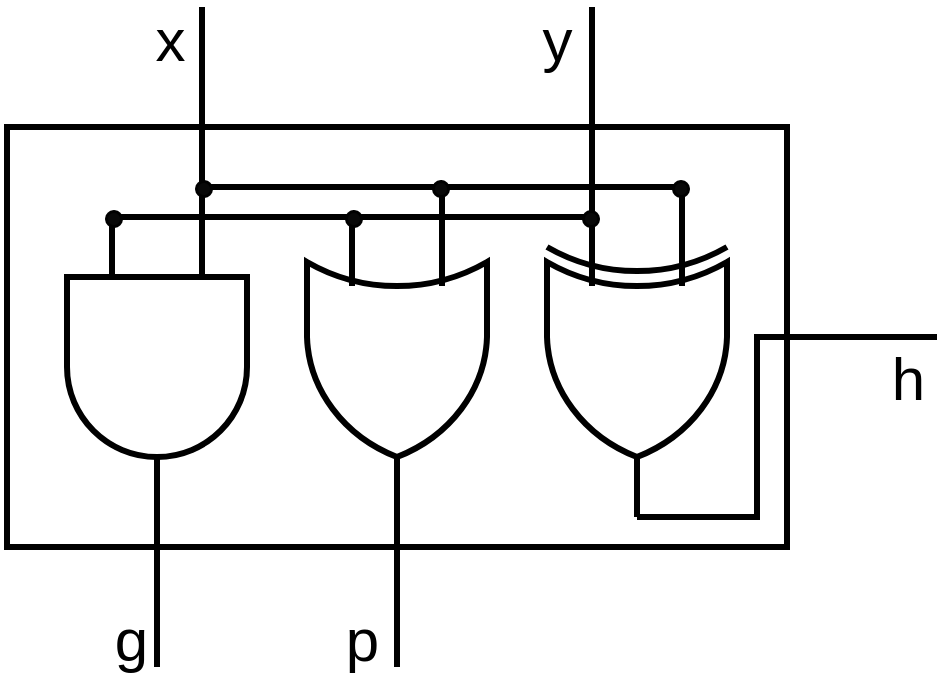
\includegraphics[width=0.5\linewidth]{diagrams/pg_block.png}
\caption{Schemat bloku PG}\label{fig:diagram_pg}
\end{figure}

\subsubsection{Blok PG\_IN}
\label{section:pg-in-block}
Blok PG\_IN jest szczególnym przypadkiem bloku PG. Pozwala on na wczesne włączenie korekty wejściowej (c\_in) do sumatora. Funkcje logiczne opisujące wyjścia tego układu zostały opisane we wzorze nr \ref{formula:pg-in}.

\begin{equation}
    \begin{cases}
      g = (x * y) + (c_{in} * (x + y))\\
      p = x\oplus y\oplus c_{in}
    \end{cases}       
    \label{formula:pg-in}
\end{equation}

\begin{figure}[H]
\centering
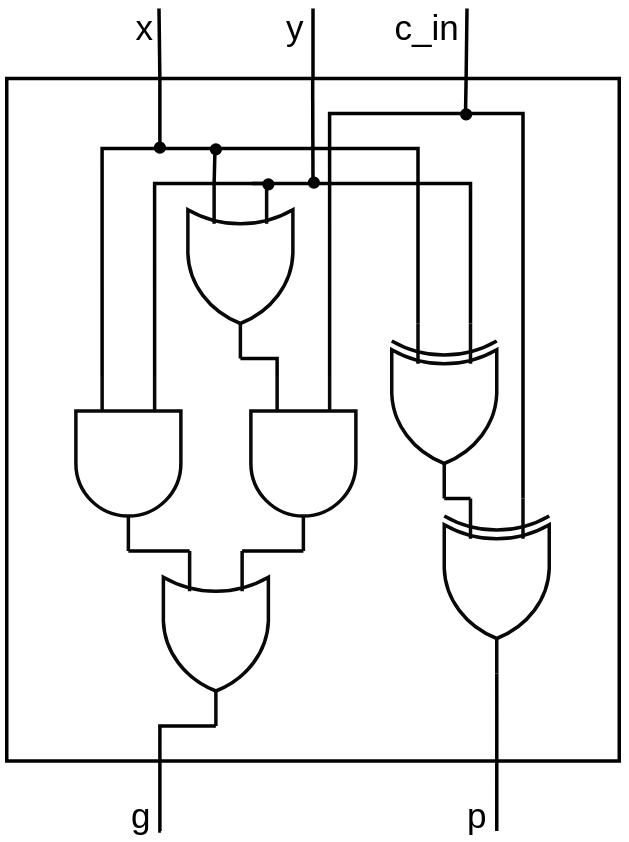
\includegraphics[width=0.5\linewidth]{diagrams/pg_in_block.png}
\caption{Schemat bloku PG\_IN}\label{fig:diagram_pg_in}
\end{figure}

\subsubsection{Węzeł sieci grafu prefiksowego}
\label{section:prefix-node}
Układ ten realizuje funkcję wektorową, opisaną wzorem nr \ref{formula:prefix-node}. Funkcje opisujące poszczególne wyjścia, zostały opisane na wzorze nr \ref{formula:prefix-node-split}. 

\begin{equation}
    \begin{cases}
        G_{H:L} = G_H + (P_H * G_L) \\
        P_{H:L} = P_H * P_L
    \end{cases}       
    \label{formula:prefix-node-split}
\end{equation}


\begin{figure}[H]
\centering
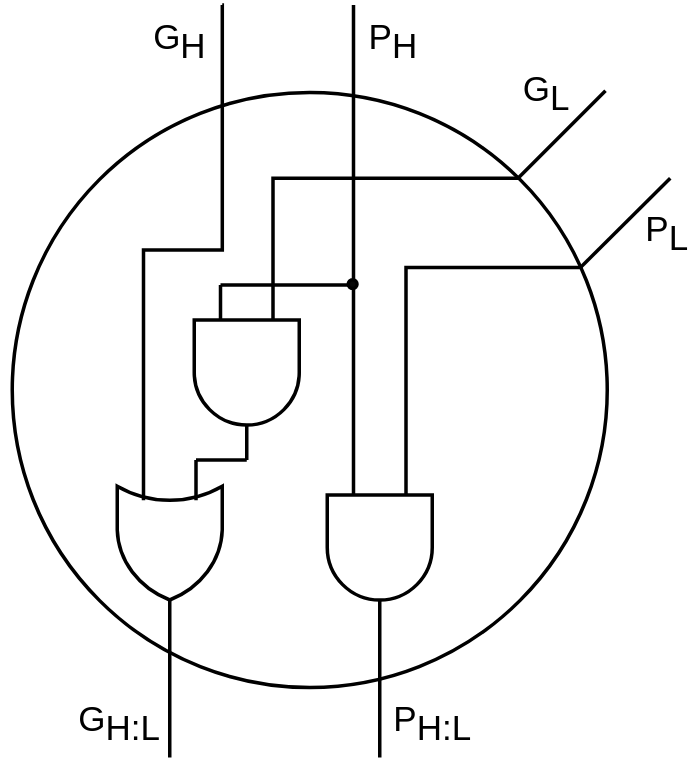
\includegraphics[width=0.5\linewidth]{diagrams/prefix_node.png}
\caption{Schemat węzła sieci grafu prefiksowego.}\label{fig:diagram_prefix_node}
\end{figure}

\subsubsection{Sumator prefiksowy}
Do zaprojektowania układu została wykorzystana architektura Ladnera-Fischera (Sklansky’ego) \cite{szybkie-sumatory-2006}. Sygnały wejściowe oraz wyjściowe, zostały opisane wzorem nr \ref{formula:prefix-adder-in-out}.

\begin{equation}
    \begin{cases}
        X = \{x_5, x_4, ..., x_0\} \\
        Y = \{y_5, y_4, ..., y_0\} \\
        S = \{s_6, s_5, ..., s_0\} = X + Y + c_{in}
    \end{cases}
    \label{formula:prefix-adder-in-out}
\end{equation}

\begin{figure}[H]
\centering
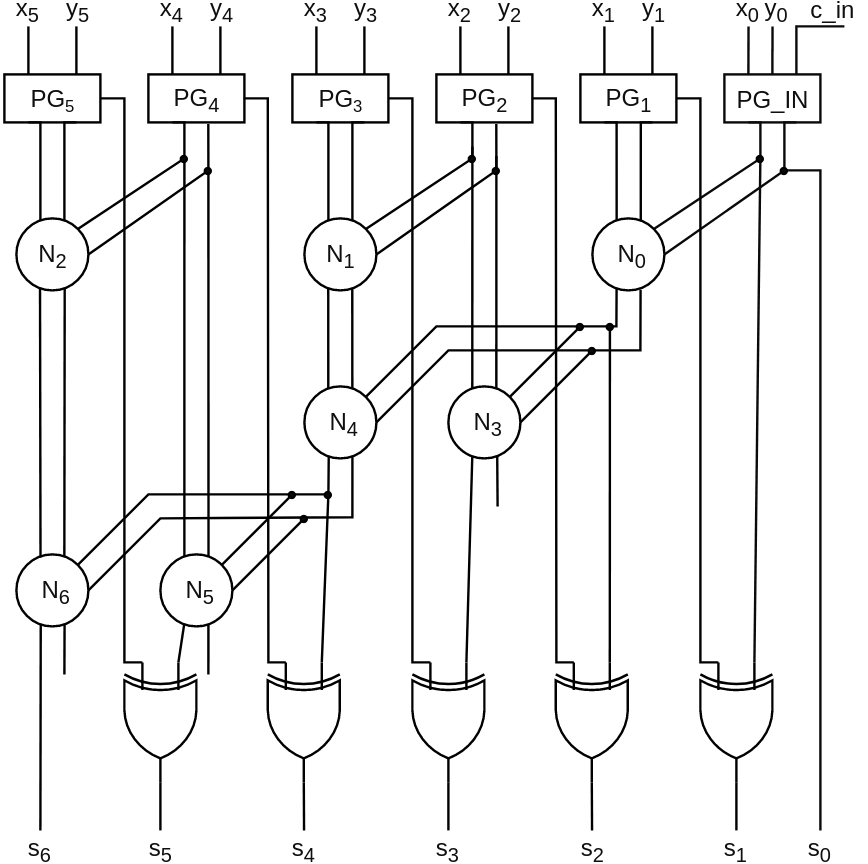
\includegraphics[width=\linewidth]{diagrams/prefix_adder.png}
\caption{Schemat układu 6-bitowego sumatora prefiksowego.}\label{fig:diagram_prefix_adder}
\end{figure}


\clearpage
\subsection{Implementacja układu za pomocą języka Verilog}
Układy z sekcji \ref{section:pg-block}, \ref{section:pg-in-block}, \ref{section:prefix-node}, zostały zrealizowane jako niezależne moduły Verilog. Dopiero moduł \textit{prefix\_adder} łączy je w 6-bitowy układ sumatora prefiksowego.

Kod bloków PG i węzłów, przedstawiony na listingach \ref{lst:module-pg}, \ref{lst:module-pg-in}, \ref{lst:module-prefix-node}, całkowicie pokrywa się z zaprezentowanymi wcześniej schematami. Moduły zawierają identyczne porty co na rysunkach \ref{fig:diagram_pg}, \ref{fig:diagram_pg_in}, \ref{fig:diagram_prefix_node}, odpowiednio zdefiniowane w kodzie jako wejście lub wyjście (\textit{input}, \textit{output}). Odpowiednie operatory określają bramki logiczne, np. "\&" dla bramki logicznej AND.

\begin{lstlisting}[caption={Moduł PG}, label={lst:module-pg}, language=Verilog]
module pg (
    input x, y,
    output gen, prop, half_sum
);

assign gen = x & y;
assign prop = x | y;
assign half_sum = x ^ y;

endmodule
\end{lstlisting}

\begin{lstlisting}[caption={Moduł PG\_IN}, label={lst:module-pg-in}, language=Verilog]
module pg_in (
    input x, y, c_in, 
    output gen, prop
);

assign gen = (x & y) | (c_in & (x | y));
assign prop = x ^ y ^ c_in;

endmodule
\end{lstlisting}

\begin{lstlisting}[caption={Moduł węzła}, label={lst:module-prefix-node}, language=Verilog]
module prefix_node (
    input gen_high, prop_high, gen_low, prop_low,
    output gen_out, prop_out
);

assign gen_out = gen_high | (prop_high & gen_low);
assign prop_out = prop_high & prop_low;

endmodule
\end{lstlisting}

\clearpage
Kod sumatora jest bardziej złożony. Został przedstawiony na listingu 4. Moduł zawiera dwa wektory sygnałów wejściowych, \textit{X} i \textit{Y} dla dodawanych liczb, sygnał przeniesienia z niższej pozycji \textit{c\_in} oraz wektor sygnałów wyjściowych dla otrzymanej sumy \textit{S}.

W liniach 17-23 zostały zadeklarowane wektory typu \textit{wire}, pełniące funkcje połączeń przewodzących sygnały pomiędzy elementami aktywnymi (bramkami).

Używanie zaimportowanych modułów przypomina korzystanie z funkcji w językach programowania. Składnia wygląda następująco:

$module\ name(.port(sygnal), ...)$,

\noindent gdzie \textit{module} to nazwa zaimportowanego modułu, \textit{name} to unikalna nazwa instancji, \textit{port} to nazwa portu w zaimportowanym module, a \textit{sygnal} to sygnał z obecnego modułu (tak jak naszym obecnym modułem jest sumator). Przykład użycia zewnętrznego modułu widać na przykład w linijce 25 listingu \ref{lst:module-prefix-adder}.
Moduły  użyte w liniach 25-39 odpowiadają za sygnały wchodzące i wychodzące do bloków PG. widać to szczególnie dobrze, gdy porównuje się kod bezpośrednio ze schematem sumatora na rysunku \ref{fig:diagram_prefix_adder}.

Moduły zaczynające się w lini 42 to węzły grafu prefiksowego. Moduł \textit{prefix\_node\_x} odpowiada węzłowi \textit{$N_x$} z rysunku \ref{fig:diagram_prefix_adder}, gdzie $ x \in [0,6]\ \land\ x \in \mathbb{N} $.

%$ x \in [0;6] \land x \in \N  $

Za przykład niech posłuży \textit{prefix\_node\_3}. Węzeł ten przyjmuje wyjścia z bloku PG na pozycji 2 oraz wyjścia z węzła 0, a następnie wyprowadza swoje wyjścia na \textit{node\_out\_g[3]} i \textit{node\_out\_p[3]}.

Na koniec wyznaczane są bity wektora wyjściowego \textit{S}. Są to proste operacje XOR z bitów pół-sumy i sygnałów generacji przeniesienia z niższej pozycji (może to być sygnał wyjściowy z konkretnego węzła lub bloku). Wyjątkiem jest najmłodszy bit sumy, będący propagacją z bloku PG\_IN.

\begin{lstlisting}[caption={Moduł sumatora prefiksowego}, label={lst:module-prefix-adder}, language=Verilog]
`include "pg.v"
`include "pg_in.v"
`include "prefix_node.v"

module prefix_adder (
    X, Y, c_in, S
);

input [5:0] X;
input [5:0] Y;
input c_in;

// Sum
output [6:0] S;

// PG block outputs, p - propagation, g - generation, h - half sum.
wire [5:0] pg_out_p;
wire [5:0] pg_out_g;
wire [5:0] pg_out_h;

// Prefix graph nodes outputs, p - propagation, g - generation.
wire [6:0] node_out_p;
wire [6:0] node_out_g;

pg_in pg_in_block(
    .x(X[0]), 
    .y(Y[0]), 
    .c_in(c_in),
    .gen(pg_out_g[0]), 
    .prop(pg_out_p[0])
);

pg pg_blocks[5:1] (
    .x(X[5:1]), 
    .y(Y[5:1]), 
    .gen(pg_out_g[5:1]), 
    .prop(pg_out_p[5:1]),
    .half_sum(pg_out_h[5:1])
);

// Instantiate prefix graph nodes.
prefix_node prefix_node_0(
    .gen_high(pg_out_g[1]),
    .prop_high(pg_out_p[1]), 
    .gen_low(pg_out_g[0]), 
    .prop_low(pg_out_p[0]),
    .gen_out(node_out_g[0]),
    .prop_out(node_out_p[0])
);
prefix_node prefix_node_1(
    .gen_high(pg_out_g[3]),
    .prop_high(pg_out_p[3]), 
    .gen_low(pg_out_g[2]), 
    .prop_low(pg_out_p[2]),
    .gen_out(node_out_g[1]),
    .prop_out(node_out_p[1])
);
prefix_node prefix_node_2(
    .gen_high(pg_out_g[5]),
    .prop_high(pg_out_p[5]), 
    .gen_low(pg_out_g[4]), 
    .prop_low(pg_out_p[4]),
    .gen_out(node_out_g[2]),
    .prop_out(node_out_p[2])
);
prefix_node prefix_node_3(
    .gen_high(pg_out_g[2]),
    .prop_high(pg_out_p[2]), 
    .gen_low(node_out_g[0]), 
    .prop_low(node_out_p[0]),
    .gen_out(node_out_g[3]),
    .prop_out(node_out_p[3])
);
prefix_node prefix_node_4(
    .gen_high(node_out_g[1]),
    .prop_high(node_out_p[1]), 
    .gen_low(node_out_g[0]), 
    .prop_low(node_out_p[0]),
    .gen_out(node_out_g[4]),
    .prop_out(node_out_p[4])
);
prefix_node prefix_node_5(
    .gen_high(pg_out_g[4]),
    .prop_high(pg_out_p[4]), 
    .gen_low(node_out_g[4]), 
    .prop_low(node_out_p[4]),
    .gen_out(node_out_g[5]),
    .prop_out(node_out_p[5])
);
prefix_node prefix_node_6(
    .gen_high(node_out_g[2]),
    .prop_high(node_out_p[2]), 
    .gen_low(node_out_g[4]), 
    .prop_low(node_out_p[4]),
    .gen_out(node_out_g[6]),
    .prop_out(node_out_p[6])
);

// Assign S output values.
assign S[0] = pg_out_p[0];
assign S[1] = pg_out_h[1] ^ pg_out_g[0];
assign S[2] = pg_out_h[2] ^ node_out_g[0];
assign S[3] = pg_out_h[3] ^ node_out_g[3];
assign S[4] = pg_out_h[4] ^ node_out_g[4];
assign S[5] = pg_out_h[5] ^ node_out_g[5];
assign S[6] = node_out_g[6];

endmodule
\end{lstlisting}


\clearpage
\subsection{Testy jednostkowe}

Testy jednostkowe modułów Verilog zostały zrealizowane za pomocą symulatora Icarus Verilog \cite{iverilog} oraz frameworku pytest \cite{pytest}. Moduły zostały przetestowane dla wszystkich możliwych wektorów sygnałów wejściowych. 

W celu zachowania przejrzystości dokumentacji, został omówiony jedynie proces testowania modułu sumatora prefiksowego. Testowanie pozostałych modułów odbywa się analogicznie.

\begin{table}[H]
\centering
\caption{Liczba przypadków testowych przypadających na moduł Verilog.}
\begin{tabular}{l|l}
\textbf{Moduł Verilog} & \textbf{Liczba przypadków testowych} \\ \hline
pg                     & $2^2 = 4$         \\ \hline
pg\_in                 & $2^3 = 8$         \\ \hline
prefix\_node           & $2^4 = 16$        \\ \hline
prefix\_adder          & $2^{13} = 8192$    
\end{tabular}
\label{table:test-case-count-per-module}
\end{table}

\subsubsection{Testbenche Verilog}
Symulacja działania modułów odbyła się poprzez utworzenie instacji testowanej jednostki z poziomu przynależącego do niej testbencha, a następnie sekwencyjne podanie wszystkich mozliwych wektorów sygnałów wejściowych. Przy każdym przebiegu pętli zadającej sygnały wejściowe, stan wejść oraz wynikających z nich wyjść, był zapisywany jako ciąg znaków, zgodny ze składnią formatu JSON.

\begin{lstlisting}[caption={Testbench dla modułu prefix\_adder}, label={lst:tb-pg}, language=Verilog]
`include "prefix_adder.v"

module prefix_adder_tb;

reg [5:0] X;
reg [5:0] Y;
reg c_in;

wire [6:0] S;

parameter TEST_SIGNAL_COUNT = 2 ** (13);

initial begin 
    $monitor (
        "{\"time\": \"%t\", \"X\": \"%6b\", \"Y\": \"%6b\", \"c_in\":\"%b\", \"S\": \"%6b\"}", 
        $time, X, Y, c_in, S
    );

    for(int i=0; i<TEST_SIGNAL_COUNT; i=i+1) begin
        {X, Y, c_in} = i;
        #1;
    end
    
    #1 $finish;
end

// UUT
prefix_adder U0 (
    .X(X),
    .Y(Y),
    .c_in(c_in),
    .S(S)
);

endmodule
\end{lstlisting}

Testbenche były syntezowane i symulowane zgodnie ze standardem  SystemVerilog 2012. Wybór tej wersji wynika z dodania wsparcia dla pętli for, która umożliwiła uproszczenie kodu i ograniczyła możliwości popełnienia błędów w jego pisaniu.

\begin{lstlisting}[caption={Przykładowe wywołanie symulacji testbencha za pomocą programu Icarus Verilog.}, label={lst:iverilog-tb-run}]
iverilog -Wall -g2012 -o ../test/pg.out tb_prefix_adder.v
\end{lstlisting}

\begin{lstlisting}[caption={Początkowy fragment treści wynikowej wywołania testbencha dla modułu prefix\_adder}, label={lst:tb-pg-json}]
{"time": "0", "X": "000000", "Y": "000000", "c_in":"0", "S": "0000000"}
{"time": "1", "X": "000000", "Y": "000000", "c_in":"1", "S": "0000001"}
{"time": "2", "X": "000000", "Y": "000001", "c_in":"0", "S": "0000001"}
{"time": "3", "X": "000000", "Y": "000001", "c_in":"1", "S": "0000010"}
{"time": "4", "X": "000000", "Y": "000010", "c_in":"0", "S": "0000010"}
{"time": "5", "X": "000000", "Y": "000010", "c_in":"1", "S": "0000011"}
{"time": "6", "X": "000000", "Y": "000011", "c_in":"0", "S": "0000011"}
{"time": "7", "X": "000000", "Y": "000011", "c_in":"1", "S": "0000100"}
{"time": "8", "X": "000000", "Y": "000100", "c_in":"0", "S": "0000100"}
\end{lstlisting}

\clearpage
\subsubsection{Testy jednostkowe pytest}
Wynik wywołania testbencha (listing \ref{lst:tb-pg-json}) był parsowany, a następnie były określane wartości oczekiwane, dla dostarczonych wartości wejściowych.

\begin{lstlisting}[caption={Test jednostkowy pytest, dla modułu prefix\_adder}, label={lst:pytest-pg}, language=Python]
@pytest.mark.parametrize("entry", data_prefix_adder)
def test_prefix_adder(entry):
    out_sum = entry["S"]
    arg_x = entry["X"]
    c_in = entry["c_in"]
    arg_y = entry["Y"]

    assert out_sum == arg_x + arg_y + c_in, "Invalid sum: {}".format(entry)
\end{lstlisting}

Test z listingu \ref{lst:pytest-pg}, dla poprawnie działającego modułu PG, daje wynik przedstawiony na listingu \ref{lst:pytest-run-pg}.

\begin{lstlisting}[caption={Wynik wywołania testów pytest dla modułu prefix\_adder.}, label={lst:pytest-run-pg}]
collected 8220 items / 28 deselected / 8192 selected                    

test/test_tb_outputs.py::test_prefix_adder[entry0] PASSED         [  0%]
test/test_tb_outputs.py::test_prefix_adder[entry1] PASSED         [  0%]
test/test_tb_outputs.py::test_prefix_adder[entry2] PASSED         [  0%]
test/test_tb_outputs.py::test_prefix_adder[entry3] PASSED         [  0%]
(8186 pominietych linii)
test/test_tb_outputs.py::test_prefix_adder[entry8190] PASSED      [ 99%]
test/test_tb_outputs.py::test_prefix_adder[entry8191] PASSED      [100%]

================= 8192 passed, 28 deselected in 45.25s ==================
\end{lstlisting}

\clearpage
\subsection{Synteza za pomocą narzędzi Yosys i Qflow}


Do syntezy układu zostały wykorzystane programy wymienione w tabeli \ref{program-versions}.

\begin{table}[H]
\centering
\caption{Wersje programów użytych do syntezy układu.}
\begin{tabular}{l|l}
\textbf{Narzędzie} & \textbf{Wersja} \\ \hline
Qflow              & 1.3r17          \\ \hline
Yosys              & 0.9-1build2     \\ \hline
Graywolf           & 0.1.6-3         \\ \hline
Qrouter            & 1.4.71.T        \\ \hline
Magic              & 8.2.157         \\ \hline
NetGen             & 1.5.133         \\ \hline
Icarus Verilog     & 10.3   
\end{tabular}
\label{program-versions}
\end{table}

Wybrana technologia wykonania układu to "osu018". Jej wybór wynika z łatwej dostępności wymaganych bibliotek (są dostarczone wraz z narzędziem qflow). Określa ona właściwości fizyczne układu wynikowego, takie jak szybkość, wymagana powierzchnia, zużycie energii.

W procesie syntezy zostały wykonane sekwencyjnie następujące kroki:
\begin{enumerate}
    \item synthesize - synteza modułu Verilog za pomocą programu yosys,
    \item place - rozmieszczenie komórek i pinów,
    \item buffer - zmniejszenie obciążalności wyjść układu,
    \item route - trasowanie ścieżek,
    \item sta - statyczna analiza czasowa,
    \item migrate - rozplanowanie przestrzenne elementów, określenie list połączeń,
    \item drc - sprawdzenie zgodności układu z regułami projektowymi,
    \item lvs - sprawdzenie zgodności układu ze schematem,
    \item gdsii - utworzenie masek w formacie GDSII, opisujących powierzchnię warstw układu \cite{gdsii},
    \item clean - usunięcie plików tymczasowych w katalogach wyjściowych.
\end{enumerate}

\clearpage
Zadanie syntezy zostało zautomatyzowane za pomocą narzędzia GNU Make \cite{gnumake}. Dzięki temu, sekwencję kroków syntezy można wywołać poleceniem "make qflow\_custom" z powłoki systemowej.

\begin{lstlisting}[caption={Fragment pliku Makefile, realizujący syntezę modułu prefix\_adder.}, label={lst:makefile-qflow}]
QFLOW_TECH = 'osu018'
QFLOW_TARGET_MODULE = 'prefix_adder'

qflow_custom: qflow_dirs
	qflow synthesize --tech $(QFLOW_TECH) $(QFLOW_TARGET_MODULE)
	qflow place --tech $(QFLOW_TECH) $(QFLOW_TARGET_MODULE)
	qflow buffer --tech $(QFLOW_TECH) $(QFLOW_TARGET_MODULE)
	qflow route --tech $(QFLOW_TECH) $(QFLOW_TARGET_MODULE)
	qflow sta --tech $(QFLOW_TECH) $(QFLOW_TARGET_MODULE)
	qflow migrate --tech $(QFLOW_TECH) $(QFLOW_TARGET_MODULE)
	qflow drc --tech $(QFLOW_TECH) $(QFLOW_TARGET_MODULE)
	qflow lvs --tech $(QFLOW_TECH) $(QFLOW_TARGET_MODULE)
	qflow gdsii --tech $(QFLOW_TECH) $(QFLOW_TARGET_MODULE)
	qflow clean --tech $(QFLOW_TECH) $(QFLOW_TARGET_MODULE)
	
qflow_dirs:
	mkdir -p synthesis layout log reports
\end{lstlisting}

\section{Wyniki i dyskusja}
\subsection{Testy i synteza}
Zaprojektowany sumator działa poprawnie. Moduły napisane w języku Verilog pomyślnie przeszły kompilację oraz zwracały właściwe wyniki podczas testowania w symulatorze. Przeprowadzony później test wyczerpujący, również zakończył się całkowitym powodzeniem. Jego wynik można zobaczyć na rysunku \ref{fig:pytest_all}.

Udało się również przeprowadzić pełną syntezę, zarówno logiczną jak i fizyczną. Powstały w ten sposób układ prezentuje rysunek \ref{fig:layout-prefix-adder}.

\begin{figure}[H]
\centering
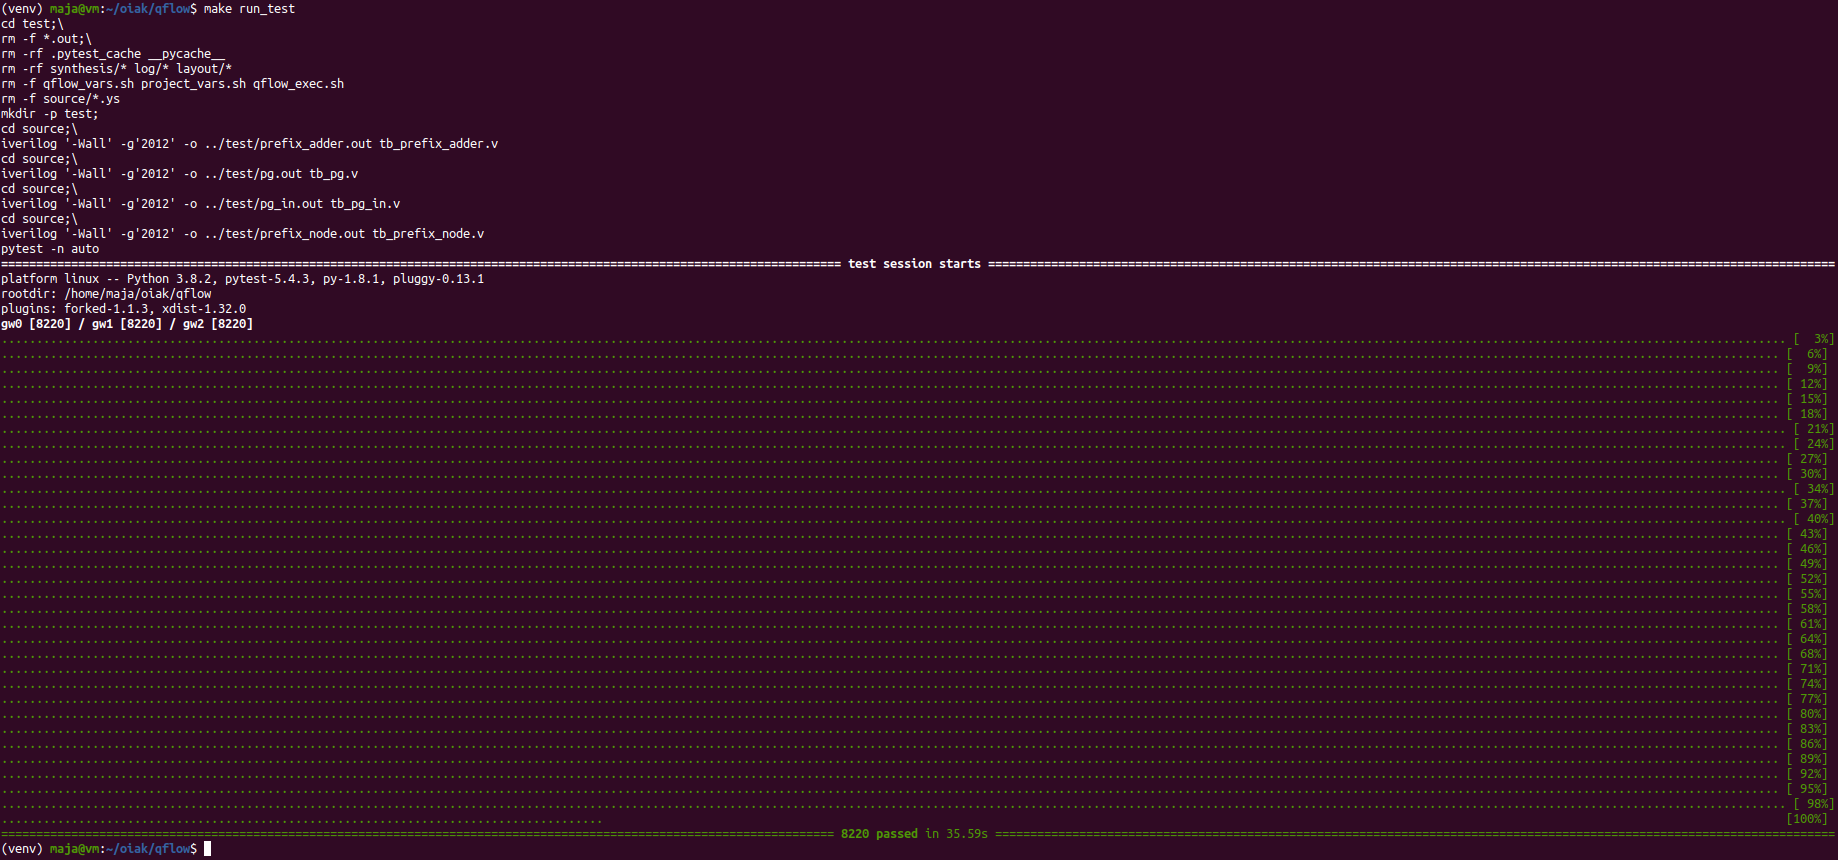
\includegraphics[width=\linewidth]{images/pytest_all.png}
\caption{Wynik testu dla sumatora}
\label{fig:pytest_all}
\end{figure}

\begin{figure}[H]
\centering
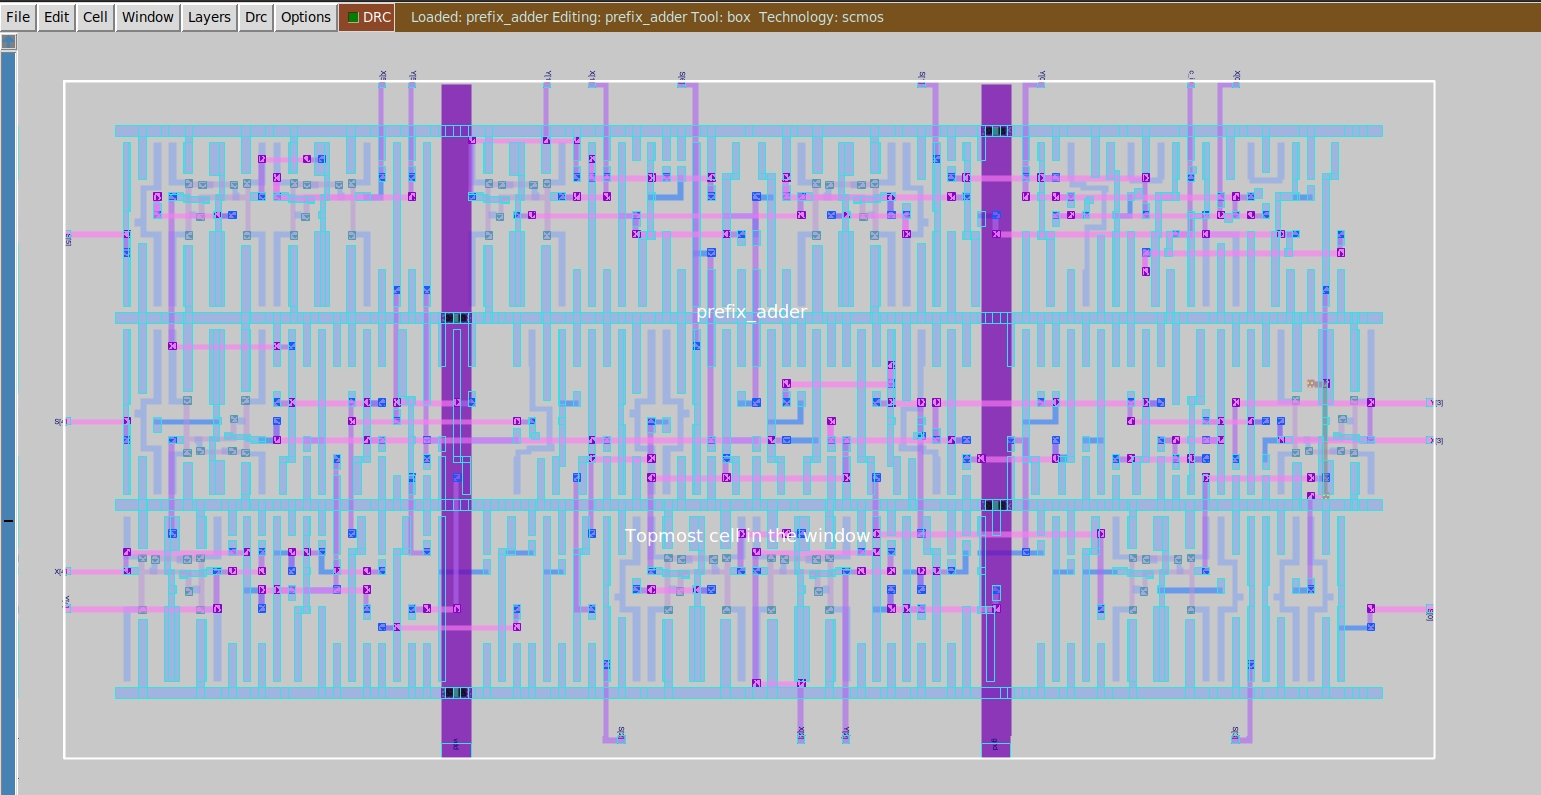
\includegraphics[width=\linewidth]{images/hardware_layout.png}
\caption{Topografia układu implementującego moduł prefix\_adder.}
\label{fig:layout-prefix-adder}
\end{figure}

\clearpage
\subsection{Statyczna analiza czasowa}
Statyczna analiza czasowa została przeprowadzona za pomocą narzędzia qflow. Wywołanie odpowiedniego polecenia oraz fragment wyniku został umieszczony na listingu \ref{lst:sta-max}.

\begin{lstlisting}[caption={Wywołanie oraz fragment wyniku statycznej analizy czasowej.}, label={lst:sta-max}]
$ qflow sta prefix_adder
(czesc tresci pominieta dla zachowania czytelnosci)
Top 0 maximum delay paths:
Computed maximum clock frequency (zero margin) = inf MHz
-----------------------------------------

Number of paths analyzed:  0

Top 0 minimum delay paths:
Design meets minimum hold timing.
-----------------------------------------

Number of paths analyzed:  7

Top 7 maximum delay paths:
Path input pin Y[0] to output pin S[5] delay 1041.84 ps
      0.0 ps                   Y[0]:              ->  AOI21X1_1/A
     93.5 ps                   _14_:  AOI21X1_1/Y ->   NOR2X1_7/B
    212.2 ps        pg_in_block_gen:   NOR2X1_7/Y ->  NAND2X1_7/A
    301.7 ps                   _17_:  NAND2X1_7/Y ->  NAND2X1_8/B
    438.0 ps  prefix_node_0_gen_out:  NAND2X1_8/Y -> NAND2X1_15/A
    534.6 ps                   _25_: NAND2X1_15/Y -> NAND2X1_16/B
    672.6 ps  prefix_node_4_gen_out: NAND2X1_16/Y -> NAND2X1_17/A
    769.3 ps                   _27_: NAND2X1_17/Y -> NAND2X1_18/B
    864.7 ps  prefix_node_5_gen_out: NAND2X1_18/Y ->   XOR2X1_5/A
    961.0 ps                 _0__5_:   XOR2X1_5/Y ->    BUFX2_6/A
   1041.8 ps                   S[5]:    BUFX2_6/Y -> S[5]
\end{lstlisting}

Na podstawie listingu \ref{lst:sta-max}, można określić minimalny czas wymagany do uzyskania poprawnego wyniku na wyjściach układu, od momentu zadania sygnałów wejściowych. Ścieżką układu wymagającą najwięcej czasu jest ścieżka $Y[0] \rightarrow S[5]$. Czas propagacji sygnału przez całą jej długość, wynosi 1041.84ps, zatem takie jest opóźnienie sygnału dla całego układu sumatora.


\section{Wnioski}
Udało się zrealizować wszystkie cele projektu. Wybrano architekturę sumatora prefiksowego i zapisano ją w języku Verilog. Zaimplementowano test wyczerpujący, z wykorzystaniem frameworku pytest, który zakończył się powodzeniem. Przeprowadzono równiż syntezę logiczną i fizyczną z pomocą narzędzi Yosys i Qflow. Cały proces został zautomatyzowany za pomocą narzędzia GNU Make, co znacząco ułatwia jego powtórne przeprowadzenie.

\bibliographystyle{unsrt}
\begin{thebibliography}{9}
    \bibitem{ubuntu}
    \href{https://ubuntu.com/}{
        System operacyjny Ubuntu\\
        \url{https://ubuntu.com/}
    }
    \bibitem {ieee-verilog}
    \href{http://staff.ustc.edu.cn/~songch/download/IEEE.1364-2005.pdf}{
        IEEE Standard for Verilog Hardware Description Language \\
        \url{http://staff.ustc.edu.cn/~songch/download/IEEE.1364-2005.pdf}
    }
    \bibitem{iverilog}
    \href{http://iverilog.icarus.com/}{
        Icarus Verilog\\
        \url{http://iverilog.icarus.com/}
    }
    \bibitem{pytest}
    \href{https://docs.pytest.org/en/stable/}{
        pytest\\
        \url{https://docs.pytest.org/en/stable/}
    }
    \bibitem{yosys} \href{http://www.clifford.at/yosys/}{
        Yosys Open Synthesis Suite\\
        \url{http://www.clifford.at/yosys/}
    }
    \bibitem{qflow}
    \href{http://opencircuitdesign.com/qflow/}{
        Qflow 1.3: An Open-Source Digital Synthesis Flow\\
        \url{http://opencircuitdesign.com/qflow/}
    }
    \bibitem{szybkie-sumatory-2009} \href{https://www.lucc.pl/inf/architektura_komputerow_1/2009_-_7_szybkie_sumatory.pdf}{
         Janusz Biernat, AK1-7-09 Szybkie sumatory.doc, 4 listopada 2009\\
        \url{https://www.lucc.pl/inf/architektura\_komputerow\_1/2009_-_7_szybkie_sumatory.pdf}
    }
    \bibitem{szybkie-sumatory-2006} \href{https://www.lucc.pl/inf/architektura_komputerow_1/2006_-_szybkie_sumatory.pdf}{Janusz Biernat, 10-06-Szybkie sumatory.doc ,2 października 2006\\
    \url{https://www.lucc.pl/inf/architektura_komputerow_1/2006_-_szybkie_sumatory.pdf}
    }
    \bibitem{yosys-manual} \href{http://www.clifford.at/yosys/files/yosys_manual.pdf}{
    Clifford Wolf, "Yosys Manual", str 14\\
    \url{http://www.clifford.at/yosys/files/yosys_manual.pdf}
    }, 
    \bibitem{opencircuitdesign-qflow} \href{http://opencircuitdesign.com/qflow/reference.html}{
        Qflow 1.4 Digital Synthesis Flow Reference Page\\
        \url{http://opencircuitdesign.com/qflow/reference.html}
    }
    \bibitem{gnumake}
    \href{https://www.gnu.org/software/make/}{
    GNU Make
    \url{https://www.gnu.org/software/make/}
    }
    \bibitem{gdsii}
    \href{https://www.rulabinsky.com/cavd/text/chapc.html}{
        Computer Aids for VLSI Design, 
        Steven M. Rubin, 
        Appendix C: GDS II Format
        \url{https://www.rulabinsky.com/cavd/text/chapc.html}
    }
\end{thebibliography}

\end{document}
